\section{Cohort Audit, Naive 2017 Critique, and Nested Hospital-Disjoint Splits}
\label{sec:cohort_splits}

\subsection{STS ACSD v2.81 Cohort and Zero-Leakage Audit}
Our cohort comprises all \textbf{368,132 isolated-CABG procedures} in STS ACSD v2.81 (1,091 U.S.\ surgical centers across nine census divisions; 100.0\% \cli{DataVrsn == 2.81}, July~1, 2014--June~30, 2017)~\cite{sts2014v281,shahian2018sts,obrien2018sts2}. Three audit corrections preceded all modeling (full schema ledger in Appendix~B):
\begin{itemize}
  \item \textbf{Skip-logic outcome reconstruction:} Under Sequence~4930, \cli{COtAFib} is populated only when the parent complication gate \cli{Complics == 1}; uncomplicated courses (\cli{Complics == 2}, 232,783 rows, 63.31\%) leave \cli{COtAFib} structurally blank. Filtering on \cli{COtAFib.notna()} induces severe collider bias~\cite{hernan2020causal}. Resolving skip logic yields \textbf{367,695 labeled cases} (437 indeterminate isolated) with \textbf{89,337 treatment-requiring POAF events (24.30\%)}. Discharge amiodarone (74.3\% vs.\ 14.7\%) and warfarin (16.5\% vs.\ 1.8\%) corroborate outcome polarity (though not an independent adjudication). Operative mortality is coded directly without the complication gate; the seven other clean auxiliary complications follow identical skip logic and are strictly quarantined from inference inputs.
  \item \textbf{Exhaustive 638 $\to$ 207 pre-incision partition:} Auditing every column against v2.81 specifications retained \textbf{207 predictors available by incision} (206 numeric/ordinal/binary indicators plus 9-level \cli{Region}). Seven hidden early-position post-operative or operative-duration fields (\cli{LOS}, \cli{PLOS}, \cli{ORDuration}, \cli{SIDuration}, \cli{SurgtoMort}, \cli{SurgtoRead}, \cli{SurgtoSternInf}) were permanently purged alongside perfusion times, discharge therapies, STS calculator outputs, and hospital/surgeon IDs. Note that STS \cli{PASYS} may be measured immediately before incision after operating-room entry.
  \item \textbf{Preoperative AF sensitivity flag:} Under v2.81 coding, \cli{ArrhythAFib == 1} denotes \emph{none}, whereas codes~2 (paroxysmal; 1,472 rows) and~3 (continuous/persistent; 428 rows) denote recorded preoperative AF (1,900 cases, 0.52\%). We retain an explicit flag rather than dropping rows, reporting sensitivity performance on the \emph{no recorded preoperative AF} subgroup ($n=21{,}103$ in holdout).
\end{itemize}

\subsection{Why Naive 2017 Splitting Is Not a Clean Statistical Comparison}
Holding out calendar year 2017 (61,552 labeled cases; 61,615 raw including 63 unlabeled rows) against 2014--2016 (306,143 labeled) is neither an external-center validation~\cite{steyerberg2016prediction,riley2019external} nor a stationary comparator (Figure~\ref{fig:split_audit}, Appendix~C):
\begin{enumerate}
  \item \textbf{99.5\% hospital overlap:} Exactly 998 of 1,003 hospitals operating in 2017 appear in 2014--2016 training (998 of 1,086 development centers, 91.9\%); only five centers are unseen.
  \item \textbf{Threefold inter-hospital POAF dispersion:} Among centers with $\ge 100$ cases, observed POAF incidence ranges from 11.7\% (5th percentile) to 34.8\% (95th percentile; SD 6.97~pp), reflecting both case mix and institutional surveillance intensity.
  \item \textbf{Half-year boundary support:} Because v2.81 ran July 2014--June 2017, 2014 covers H2 only (POAF 23.69\%) whereas 2017 covers H1 only (24.83\%, Year TV $= 1.000$), confounding calendar coverage with temporal change.
  \item \textbf{Non-stationary missingness drift:} Missingness shifted by $+6.05$~pp on \cli{LVSD}, $+6.04$~pp on \cli{LVEDD}, and $+5.60$~pp on \cli{PctStenAM}, pushing worst-case marginal standardized mean difference to $\mathrm{Max}\,|\mathrm{SMD}| = 0.2793$.
  \item \textbf{Multivariate covariate shift:} Adversarial discrimination of 2017 versus 2014--2016 reaches 0.6208 overall (0.5908 strictly hospital-grouped; 0.7661 vs.\ 2014 alone).
\end{enumerate}

\begin{figure*}[t]
  \centering
  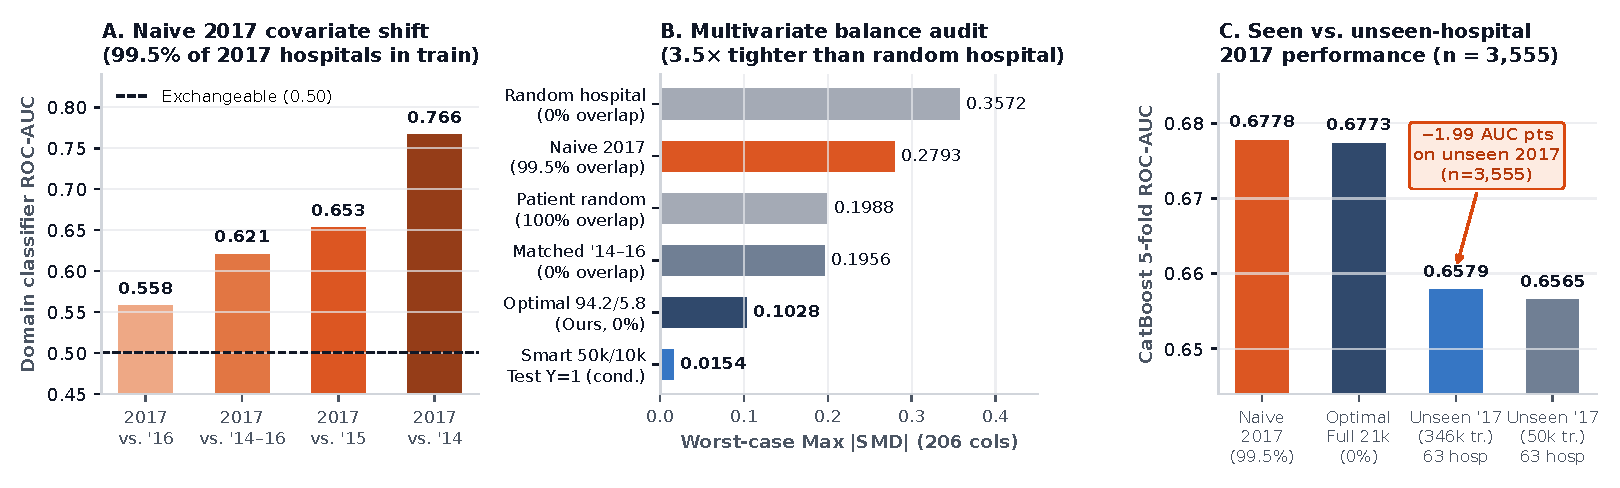
\includegraphics[width=\textwidth]{figures/fig2_2017_pathology_and_split_audit.pdf}
  \caption{\ct{Covariate balance and 2017 performance under temporal and hospital-disjoint splits.} \textbf{(A)}~Domain-classifier ROC-AUC across calendar contrasts (207 pre-incision features). \textbf{(B)}~Worst-case $|\mathrm{SMD}|$ across 206 numeric predictors for five whole-cohort split strategies plus the nested class-conditional \cli{Smart 50k/10k Test} ($Y=1$) subsample diagnostic (full metrics in Appendix~C). \textbf{(C)}~Tuned 207-feature CatBoost ROC-AUC is 0.6778 on naive 2017 (99.5\% seen centers) and is lower at 0.6579 on 2017 patients at strictly unseen hospitals ($n=3{,}555$, 63 centers).}
  \label{fig:split_audit}
\end{figure*}

\begin{callout}{Seen-hospital vs.\ unseen-hospital 2017 performance}
A matched 207-feature CatBoost architecture scores \textbf{0.6778} on the naive 2017 holdout (99.5\% familiar hospitals) versus \textbf{0.6579} on 2017 cases treated at genuinely unseen hospitals ($n=3{,}555$, 63 centers; Figure~\ref{fig:split_audit}C)---a \textbf{$-1.99$ AUC-point} difference. Because these two designs also differ in training periods and cohort membership (our optimal split includes 57,997 full or 8,446 small 2017 cases from other hospitals), this contrast evaluates \emph{within-2017 unseen-hospital transport} rather than isolating hospital familiarity alone, illustrating how sharply evaluation geometry alters apparent AUC.
\end{callout}

\subsection{Optimal 94.2/5.8 Split and Nested Smart 50k/10k Benchmark}
Random hospital-grouped splitting removes site overlap (0.0\%) but induces severe finite-cluster imbalance ($\mathrm{Max}\,|\mathrm{SMD}| = 0.3572$, Region TV $= 0.1645$, POAF gap 1.13~pp; Appendix~C). We therefore applied cluster-level multivariate anticlustering~\cite{papenberg2021anticlustering}, ranking finalists by proxy balance loss plus $50\times$ 32-D whitened SPlit Energy Distance~\cite{joseph2022split,szekely2013energy} while monitoring multi-kernel $\mathrm{MMD}^2$~\cite{gretton2012kernel} as a zero-clipped diagnostic across covariates, missingness, region, calendar year, rare Mahalanobis tails, and all nine registry outcomes subject to a $\ge 5{,}000$ holdout POAF-event floor. This partitions the 1,091 centers into \textbf{1,017 training hospitals ($N=346{,}454$; 94.2\%)} and \textbf{74 strictly unseen holdout hospitals ($N=21{,}241$; 5.8\%, 5,160 POAF events, 24.29\%)}, cutting Energy Distance 4.1$\times$ ($0.01732 \to 0.00427$), $\mathrm{Max}\,|\mathrm{SMD}|$ 3.5$\times$ ($0.3572 \to 0.1028$), Region TV 57$\times$, and Year TV 23$\times$ with 0.0\% hospital overlap. Five inner hospital-disjoint CV folds span 203--204 centers each.

Because frontier in-context Tabular Foundation Models (TFMs) operate natively over 10k--50k contexts~\cite{jaeger2026tabpfn35,qu2026kumotabular,kong2026tabfm}, we nested a balanced \textbf{50,000 / 10,000} cohort inside the exact same 1,017 / 74 hospital partition via class-conditional support-point subsampling~\cite{joseph2022split} (25k/25k train across five exact 10k hospital-disjoint folds; 5k/5k holdout test achieving zero-clipped diagnostic $\mathcal{E}_{32\mathrm{D}}=0.00000$ relative to its overlapping parent holdout). Probabilities trained on balanced 50/50 data map back to natural clinical prevalence using the closed-form development-only Bayes prior-shift offset~\cite{king2001logistic,saerens2002adjusting}:
\begin{equation}
  \operatorname{logit}\bigl(\hat{p}_{\mathrm{nat}}(x)\bigr) = \operatorname{logit}\bigl(\hat{p}_{\mathrm{bal}}(x)\bigr) - 1.136479,
  \label{eq:bayes_shift}
\end{equation}
where $1.136479 = \operatorname{logit}(0.50) - \operatorname{logit}(0.242967)$ uses strictly the development full-training prevalence. Because both the 94.2/5.8 optimizer and class-ratio weighting used label counts (without individual Horvitz--Thompson inclusion probabilities~\cite{horvitz1952generalization}), we designate the full natural-prior 74-hospital holdout (\cli{test\_full\_21k}, $N=21{,}241$) as our \textbf{primary retrospective evaluation} and the nested 10,000-row slice as a balanced context-budget sensitivity. With this leakage-free, hospital-disjoint benchmark fixed, we next test whether explicit clinical feature engineering improves unseen-hospital transport (\S\ref{sec:agentic_fe}).
